\section{Estado de la cuestión}
\label{chap:estado_cuestion}

% \defaultFontEpigraph{Diversity Is All You Need\dots}{\cite{eysenbachDiversityAllYou2018}}
% \defaultFontEpigraph{Diversity Is All You Need\dots}{Eysenbach, Gupta, Ibarz, y Levine (2018)}

En la actualidad, la generación de música o, en un sentido amplio, de sonido, constituye uno de los frentes de investigación activos y más prometedores en el campo de la IA. La generación música con modelos de \gls{dl} ha sido abordado históricamente desde dos grandes perspectivas en función de la naturaleza de los datos generados por los modelos: la generación de música simbólica y la generación de música con audio. La primera de ellas consiste en la creación de elementos musicales como notas, acordes, melodías, etc. en un formato simbólico, ya sea MIDI, OSC, MusicXML, ABC, Lilypond, o cualquier formato musical reducible a símbolos textuales. La segunda, en la creación de un flujo de audio directamente reproducible sin necesidad de síntesis sonora o utilización de bibliotecas de \textit{samples}. Encontramos investigaciones recientes en ambos campos, incluso en la combinación de ambos, donde se generan elementos simbólicos que son posteriormente convertidos a audio. La Figura \ref{fig:generacion_musica_estado_cuestion} muestra un esquema de las diferentes aproximaciones a la generación de música con \gls{ia}. Además de analizar el estado del arte en estos campos, se analizará también el uso de los \gls{llm} en la creación de código de programación, campo muy activo y que puede arrojar luz sobre el uso de estos modelos en la creación de código de lenguajes de programación musical.

\begin{figure}[H]
    \caption{Esquema de las diferentes aproximaciones a la generación de música con IA}
    \centering
    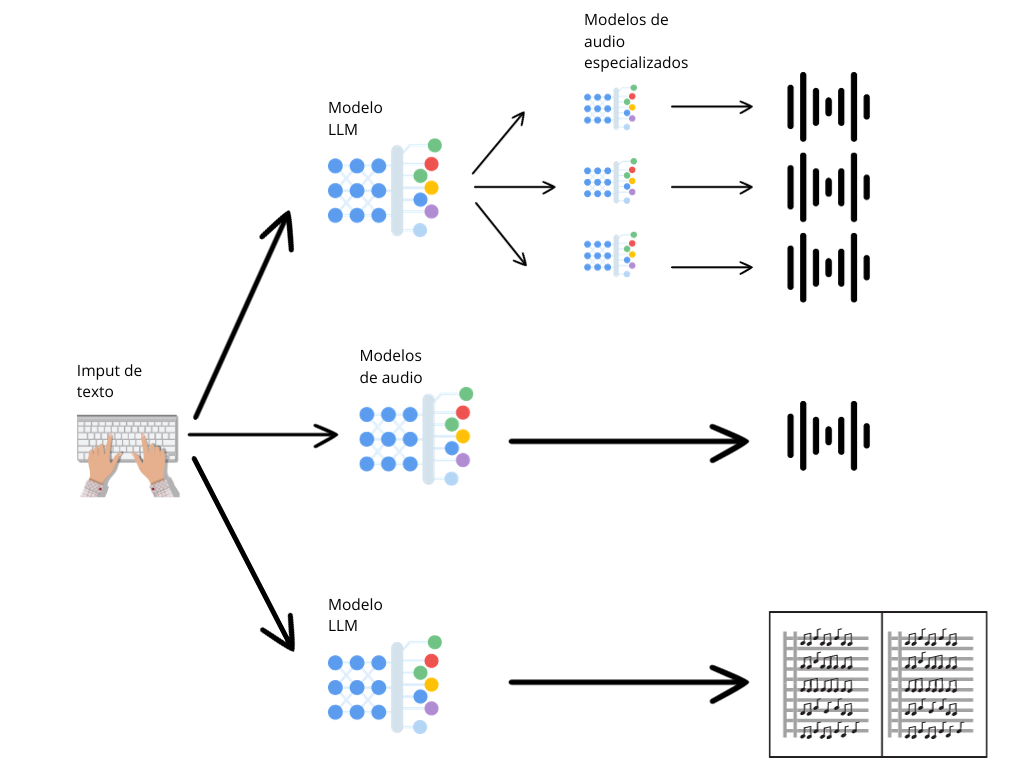
\includegraphics[width=0.7\textwidth]{./figuras/generacion_musica_estado_cuestion.png}
    \source{\propio}
    \label{fig:generacion_musica}
\end{figure}

\subsection{Modelos de IA generativa aplicados a la música}

La primera aproximación, la de la composición informática de música a través de elementos simbólicos, se remonta a los inicios de la computación, con pioneros como Lejaren Hiller y Leonard Isaacson, que en 1957 crearon \textit{Illiac Suite} \citep{arizaTwoPioneeringProjects2011,funkMusicalSuiteComposed2018}, la primera composición musical generada por ordenador. Desde entonces, la generación de música simbólica ha sido abordada desde diferentes perspectivas, como la generación de música aleatoria, la generación de música a partir de reglas, la generación de música a partir de modelos probabilísticos como las cadenas de Markov, música basada en mátemática fractal, estocástica, etc. \citep{hernandez-olivanSurveyArtificialIntelligence2022}. 

La generación de audio por medio de modelos de \gls{dl} es un campo de investigación más reciente debido en parte a su gran demanda computacional, que ha estado fuera del alcance de investigadores y empresas hasta la última década. Actualmente, modelos como \textit{MuseNet}  \citep{departmentofcomputersciencesrminstituteofscienceandtechnologychennaiindia.MusenetMusicGeneration2020a}, \textit{Jukebox} \citep{dhariwalJukeboxGenerativeModel2020}, \textit{Stable Audio} \cite{StableAudioFast}, o \textit{Suno} \citep{SunoAI}, entre otros, están consiguiendo diariamente inéditos avances en lo que se refiere a la generación de música en formato de audio de una alta calidad, y, al igual que está ocurriendo con modelos de generación de imagen o vídeo, se espera que en los próximos años se produzcan avances muy significativos en este campo.


\subsection{LLM como asistentes para la creación de música simbólica}
\label{sec:llm_asistentes_creacion_codigo_programacion}

La aproximación a la generación de música a través de elementos simbólicos en lugar de puro audio adquiere una renovada fuerza por la aparición de los \gls{llm}, los cuales se basan en la arquitectura \textit{Transformer}, aparecida en 2017 \citep{vaswaniAttentionAllYou2017}, por lo que es un tema de investigación muy reciente y al que se le está prestando menos atención. El grueso de las investigaciones candentes en este momento se están centrando en la generación de audio, campo más prometedor desde el punto de vista comercial. No obstante, existen recientes investigaciones en este campo, como \textit{MuseCoco} \citep{luMuseCocoGeneratingSymbolic2023}, que propone un procedimiento en dos etapas desde el input de texto en lenguaje natural del usuario hasta la generación de música simbólica en forma de partitura. La Figura \ref{fig:musecoco} muestra el esquema de funcionamiento de este sistema. 

\begin{figure}[H]
    \caption[Esquema de funcionamiento en dos pasos de MuseCoco texto--música]{Esquema de funcionamiento en dos pasos de MuseCoco en la generación de música simbólica desde texto}
    \centering
    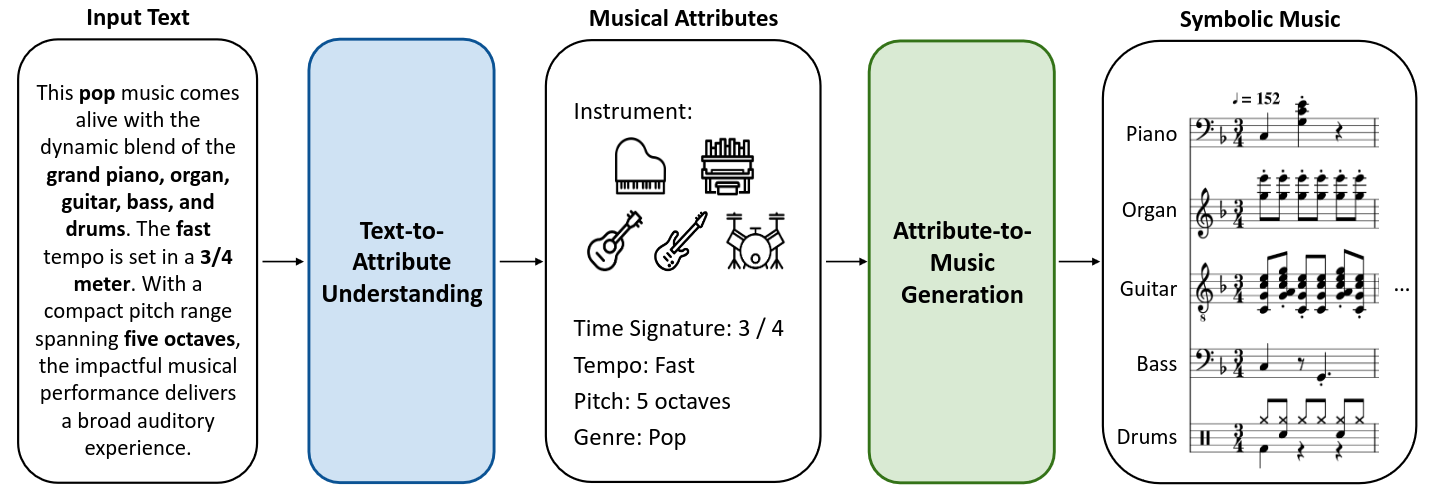
\includegraphics[width=0.9\textwidth]{./figuras/musecoco_two_steps.png}
    \source{\cite{luMuseCocoGeneratingSymbolic2023}}
    \label{fig:musecoco}
\end{figure}

Otro interesante trabajo sobre el uso de \gls{llm} para la generación musical es \textit{WavJourney} \citep{liuWavJourneyCompositionalAudio2023}, donde el papel del \gls{llm} es el de agente compositivo capaz de conectarse con otros modelos de generación de audio (voz, instrumentos, ruidos, música, etc.) para <<componer>> a partir del input o prompt del usuario. En este caso, el \gls{llm} juega un papel de mediador y planificador de la composición, además de generador de prompts para los diversos modelos implicados en la generación de audio. La Figura \ref{fig:wavjourney} muestra el esquema de funcionamiento de este sistema. Una aproximación similar en cuanto al uso de los \gls{llm} en la generación de audio lo encontramos en \cite{borsosAudioLMLanguageModeling2023}.

\begin{figure}[H]
    \caption[Esquema de funcionamiento de \textit{WavJourney}]{Esquema de funcionamiento de WavJourney en la generación de audio desde texto}
    \centering
    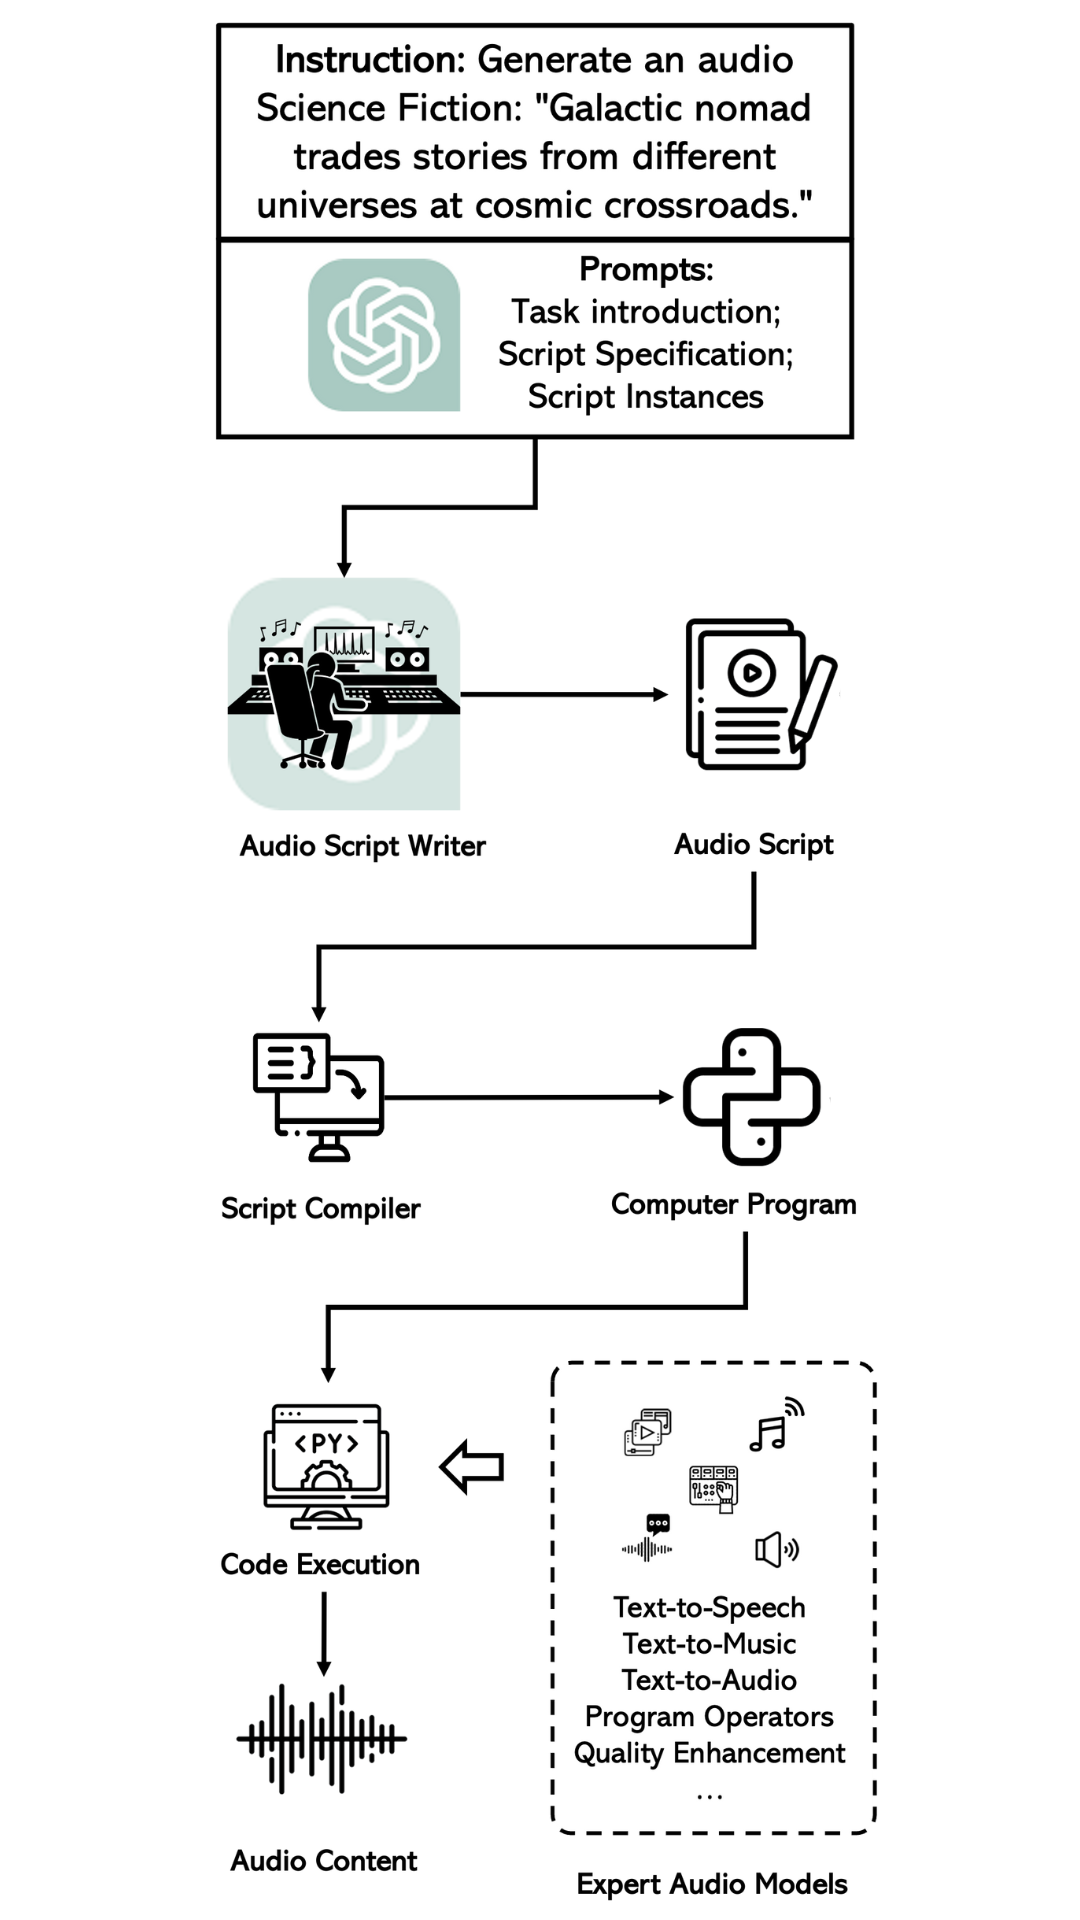
\includegraphics[width=0.4\textwidth]{./figuras/WavJourney.png}
    \source{\cite{liuWavJourneyCompositionalAudio2023}}
    \label{fig:wavjourney}
\end{figure}

\subsection{LLM en la creación de código de programación}
\label{sec:llm_creacion_codigo_programacion_estado_cuestion}

La generación de código de programación por \gls{llm}, independientemente de su finalidad artística o técnica, sí que es un campo muy estudiado en los últimos años, y que ha dado lugar a la aparición de modelos como \textit{Github Copilot}, que ha sido capaz de generar código de programación de considerable calidad a partir de inputs o \textit{prompts} en lenguaje natural. \textit{Github Copilot} es un servicio que integra un modelo GPT-4 junto a un conjunto de aplicaciones de integración en entornos de desarrollo como \textit{Visual Studio Code}, \textit{Atom}, etc. Debido a su amplia aplicación en el campo de la programación, es un modelo que ha recibido una gran atención mediática, y que ha sido objeto de numerosos estudios y análisis, por lo que podemos considerarlo como el estado del arte en la generación de código de programación por \gls{llm}. Es por ello que los principales estudios sobre la interacción de \gls{llm} con humanos en el campo de la programación se han centrado en este servicio. De todos estos artículos podemos extraer conclusiones de interés.

Se ha investigado con detalle el impacto que tiene el diseño de prompts adecuados a la tarea de generación de código. \cite{liStructuredChainofThoughtPrompting2023} llega a la conclusión de que un uso adecuado de la técnica de \textit{prompting} \gls{cot} puede mejorar significativamente la calidad y corrección del código generado. Esta variante es denominada \gls{scot}, y consiste en solicitar la respuesta del \gls{llm} en dos pasos: primero, una descripción en pseudocódigo de la tarea a realizar, y segundo, la implementación en código final de la tarea. En el estudio se muestra que el uso de \gls{scot} mejora el índice de corrección del código generado en un 13,79\% respecto al uso de \gls{cot} en lenguajes como Python o C++.

Otro estudio relevante para nuestro trabajo es \cite{chenTeachingLargeLanguage2023}, donde se analizan técnicas de \textit{Self-Debugging}, donde, por medio de \textit{few-shot}, se predispone al \gls{llm} para la autorevisión del código generado, consiguiendo una mejora de hasta el 12\%.

Un aspecto importante, además de la corrección del código generado por medio de \gls{llm}, es el impacto en la productividad de su uso en tareas concretas de programación. \citep{pengImpactAIDeveloper2023a} mostró que estas pueden llegar a realizarse un 55,8\% más rápido que sin su ayuda, aunque necesario señalar que en este estudio participaron investigadores de Microsoft, empresa que desarrolla \textit{Github Copilot}, con lo cual los resultados pueden estar sesgados. En esta línea, investigadores Montreal y Toronto, observaron que herramientas como \textit{Github Copilot} dan resultados muy comparables a los de programadores humanos, si bien su utilidad es mayor cuando lo utilizan programadores con experiencia, constituyendo cierto riesgo en manos de programadores noveles \citep{moradidakhelGitHubCopilotAI2023}. Otro interesante estudio sobre la fiabilidad de la generación de código de \textit{Github Copilot} \citep{mastropaoloRobustnessCodeGeneration2023}, halló que en casi la mitad de los casos, el código generado por dos descripciones en lenguaje natural semánticamente equivalentes, era diferente, y en más de una cuarta parte de los casos la corrección del código se vio comprometida, lo que pone en tela juicio la robustez del sistema.


